\section{Experimental Evaluation}

\begin{frame}{Implementation}
\begin{itemize}[<+->]
    \item We integrated our algorithm into the Storm Model Checker
    \item Top performing Model Checker in QComp2019 competition
    \item Supports a variety of models, including MDPs but not SMGs
    \item Large codebase with modular design
    \item Our implementation is based on a sparse matrix
    \item Modern C++ features
\end{itemize}
\uncover<+->{
Supported properties:
\[
\langle\langle C \rangle\rangle\;\mathsf{P}\vartriangle p\; [\phi_1 \, \until \, \phi_2] 
\quad\text{with}\quad\vartriangle \in \{<, \leq, =, \geq, >\}, p \in \set{0, 1}
\]
}


\iffalse
where $C$ is a coalition of players, $\vartriangle \in \{<, \leq, =, \geq, >\}$, $p \in \set{0, 1}$, and $\phi_1, \phi_2$ are subformulas. All states belonging to the specified coalition are assigned to Player $0$, while the remaining states are assigned to Player $1$.
\fi
    
\end{frame}

\begin{frame}{PRISM-games}

\begin{itemize}[<+->]
    \item First comprehensive tool for checking SMGs
    \item Initial release in 2012
    \item Written in Java
    \item Support for SMGs both explicitly and symbolically
\end{itemize}

\end{frame}

\begin{frame}{Research Questions}
    \begin{itemize}[<+->]
    \item[\textbf{RQ1}:] How does the performance of our algorithm compare to the existing implementation in PRISM-games?
    \item[\textbf{RQ2}:] How much performance gain is achieved by performing the computations symbolically?
    \item[\textbf{RQ3}:] How does the performance of our algorithm, when run on MDPs, compare to existing implementations for MDPs in PRISM-games and Storm?
    \item[\textbf{RQ4}:] How does real-world performance compare to the worst-case performance?
\end{itemize}
\end{frame}

\begin{frame}{Benchmarks: Worst Case Example (SWC)\hfill $\ASReach_0(T=\set{t_n}, \mathcal{G})$}
\centering
\begin{tikzpicture}[>=stealth, node distance=1.8cm, every node/.style={font=\small}]
    % Nodes for s chain
    \node[draw, minimum size=1cm, shape=rectangle] (S1) {$s_1$};
    \node[draw, minimum size=1cm, shape=rectangle, right=of S1] (S2) {$s_2$};
    \node[draw, minimum size=1cm, shape=rectangle, draw=none, right=of S2] (dots) {\dots};
    \node[draw, minimum size=1cm, shape=rectangle, right=of dots] (Snm1) {$s_{n-1}$};
    \node[draw, minimum size=1cm, shape=rectangle, right=of Snm1] (Sn) {$s_n$};

    % Nodes for t chain
    \node[draw, minimum size=1cm, shape=rectangle, above=1.8cm of S1] (T1) {$t_1$};
    \node[draw, minimum size=1cm, shape=rectangle, right=of T1] (T2) {$t_2$};
    \node[draw, minimum size=1cm, shape=rectangle, draw=none, right=of T2] (dotsT) {\dots};
    \node[draw, minimum size=1cm, shape=rectangle, right=of dotsT] (Tnm1) {$t_{n-1}$};
    \node[draw, minimum size=1cm, shape=rectangle, right=of Tnm1] (Tn) {\textcolor{myred}{$t_n$}};

    % Self-loops for s chain

    \draw[->] (S2) edge[loop above]
        node[above, pos=0.5] {$(s_2, a)$} 
        coordinate[pos=0.5] (S2loop) (S3);
    \filldraw[black] (S2loop) circle (2pt);
    
    \draw[->] (Snm1) edge[loop above]
        node[above, pos=0.5] {$(s_{n-1}, a)$} 
        coordinate[pos=0.5] (Snm1loop) (S3);
    \filldraw[black] (Snm1loop) circle (2pt);
    
    \draw[->] (Sn) edge[loop above]
        node[above, pos=0.5] {$(s_{n}, a)$} 
        coordinate[pos=0.5] (Snloop) (S3);
    \filldraw[black] (Snloop) circle (2pt);

    
    % t_n selfloop
    \draw[->] (Tn) edge[loop above]
        node[above, pos=0.5] {$(t_{n}, a)$} 
        coordinate[pos=0.5] (Tnloop) (S3);
    \filldraw[black] (Tnloop) circle (2pt);

    % Transitions within s chain
    \draw[-] (S1) -- node[below] {} ($(S1)!0.5!(S2)$);
    \filldraw[black] ($(S1)!0.5!(S2)$) circle (2pt) node[label={90:$(s_1, b)$}] {};
    \draw[->] ($(S1)!0.5!(S2)$) -- (S2);
    \draw[->] ($(S1)!0.5!(S2)$) .. controls +(0,-1) and +(0,-1) .. node[below] {} (S1);

    \draw[-] (S2) -- node[below] {} ($(S2)!0.5!(dots)$);
    \filldraw[black] ($(S2)!0.5!(dots)$) circle (2pt) node[label={90:$(s_2, b)$}] {};
    \draw[->] ($(S2)!0.5!(dots)$) -- (dots);
    \draw[->] ($(S2)!0.5!(dots)$) .. controls +(0,-1.5) and +(0,-1.5) .. node[below] {} (S1);

    \draw[-] (dots) -- node[below] {} ($(dots)!0.5!(Snm1)$);
    \filldraw[black] ($(dots)!0.5!(Snm1)$) circle (2pt) node[label={90:$(s_{n-2}, b)$}] {};
    \draw[->] ($(dots)!0.5!(Snm1)$) -- (Snm1);
    \draw[->] ($(dots)!0.5!(Snm1)$) .. controls +(0,-2) and +(0,-2) .. node[below] {} (S1);

    \draw[-] (Snm1) -- node[below] {} ($(Snm1)!0.5!(Sn)$);
    \filldraw[black] ($(Snm1)!0.5!(Sn)$) circle (2pt) node[label={90:$(s_{n-1}, b)$}] {};
    \draw[->] ($(Snm1)!0.5!(Sn)$) -- (Sn);
    \draw[->] ($(Snm1)!0.5!(Sn)$) .. controls +(0,-3) and +(0,-3) .. node[below] {} (S1);

    % Transitions from s chain to t chain
    \draw[-] (S1) -- node[below] {} ($(S1)!0.5!(T1)$);
    \filldraw[black] ($(S1)!0.5!(T1)$) circle (2pt) node[label={180:$(t_1, a)$}] {};
    \draw[->] ($(S1)!0.5!(T1)$) -- (T1);

    \draw[-] (T1) -- node[below] {} ($(T1)!0.5!(T2)$);
    \filldraw[black] ($(T1)!0.5!(T2)$) circle (2pt) node[label={90:$(t_2, a)$}] {};
    \draw[->] ($(T1)!0.5!(T2)$) -- (T2);

    \draw[-] (T2) -- node[below] {} ($(T2)!0.5!(dotsT)$);
    \filldraw[black] ($(T2)!0.5!(dotsT)$) circle (2pt) node[label={90:$(t_{n-2}, a)$}] {};
    \draw[->] ($(T2)!0.5!(dotsT)$) -- (dotsT);

    \draw[-] (dotsT) -- node[below] {} ($(dotsT)!0.5!(Tnm1)$);
    \filldraw[black] ($(dotsT)!0.5!(Tnm1)$) circle (2pt) node[label={90:$(t_{n-1}, a)$}] {};
    \draw[->] ($(dotsT)!0.5!(Tnm1)$) -- (Tnm1);

    \draw[-] (Tnm1) -- node[below] {} ($(Tnm1)!0.5!(Tn)$);
    \filldraw[black] ($(Tnm1)!0.5!(Tn)$) circle (2pt) node[label={90:$(t_n, a)$}] {};
    \draw[->] ($(Tnm1)!0.5!(Tn)$) -- (Tn);

\end{tikzpicture}
\end{frame}
\begin{frame}{Benchmarks: Investor (INV)}
\begin{itemize}[<+->]
    \item Taken from Case Study of Prism-Games, McIver and Morgan (2007)
    \item An investor can bet on the future price of a stock
    \item One time step later, the stock randomly changes its price and the investment is settled
    \item The stock price has a minimum and maximum
    \item The stock market can non-deterministically bar the investor for one time step
    \item In which situations can the investor almost-surely make a profit?
\end{itemize}
    
\end{frame}

\begin{frame}{Runtime Comparison for SWC}
\pgfplotsset{compat=1.18}



\begin{figure}[t]
\centering
\begin{tikzpicture}
    \begin{loglogaxis}[
        xlabel={Number of States},
        ylabel={Time (s)},
        width=8cm,
        legend pos=outer north east,
        ytick={1e-3,1e-2,1e-1,1e0,1e1,1e2}, % Regular ticks
        yticklabels={$\leq10^{-3}$,$10^{-2}$,$10^{-1}$,$10^0$,$10^1$,$10^2$},
    ]
    \addplot[myblue, mark=triangle*] table[x=number_of_states, y=storm_reachability, col sep=comma] {figures/data/bad_runtime_example.csv};
    \addlegendentry{Storm}

    \addplot[mygreen, mark=square*] table[x=number_of_states, y=prism_reachability, col sep=comma] {figures/data/bad_runtime_example.csv};
    \addlegendentry{PRISM-games}

    \only<2->{
    \addplot[mypink, mark=pentagon*] table[x=number_of_states, y=prism_symbolic_reachability, col sep=comma] {figures/data/bad_runtime_example.csv};
    \addlegendentry{PRISM-games (dd)}
    }
    \end{loglogaxis}
\end{tikzpicture}
\label{fig:plot_swc}
\end{figure}



\end{frame}
\begin{frame}{Runtime Comparison for INV}

\pgfplotsset{compat=1.18}


\begin{figure}[t]
\centering
\begin{tikzpicture}
    \begin{loglogaxis}[
        xlabel={Number of States},
        ylabel={Time (s)},
        width=8cm,
        legend pos=outer north east,
        ytick={1e-3,1e-2,1e-1,1e0,1e1}, % Regular ticks
        yticklabels={$\leq10^{-3}$,$10^{-2}$,$10^{-1}$,$10^0$,$10^1$},
    ]
    \addplot[myblue, mark=triangle*] table[x=number_of_states, y=storm_reachability, col sep=comma] {figures/data/investor.csv};
    \addlegendentry{Storm}

    \addplot[mygreen, mark=square*] table[x=number_of_states, y=prism_reachability, col sep=comma] {figures/data/investor.csv};
    \addlegendentry{PRISM-games}

    \only<2->{
    \addplot[mypink, mark=pentagon*] table[x=number_of_states, y=prism_symbolic_reachability, col sep=comma] {figures/data/investor.csv};
    \addlegendentry{PRISM-games (dd)}
    }
    \end{loglogaxis}
\end{tikzpicture}
\label{fig:plot_inv}
\end{figure}



\end{frame}
\begin{frame}{Scatter Plot of Benchmarks}
\begin{figure}[t]
\centering
\begin{tikzpicture}
    \begin{loglogaxis}[
        axis equal,
        width=8cm,
        height=8cm,
        xmin=0.0005, xmax=160,
        ymin=0.0005, ymax=160,
        xlabel={Storm (s)},
        ylabel={PRISM-games (s)},
        legend pos=outer north east,
        xtick={1e-3,1e-2,1e-1,1e0,1e1,1e2}, % Regular ticks
        xticklabels={$\leq10^{-3}$,$10^{-2}$,$10^{-1}$,$10^0$,$10^1$,$10^2$},
        ytick={1e-3,1e-2,1e-1,1e0,1e1,1e2}, % Regular ticks
        yticklabels={$\leq10^{-3}$,$10^{-2}$,$10^{-1}$,$10^0$,$10^1$,$10^2$},
    ]
    \addplot[only marks, mark=*, mark options={myorange}] table[x=storm_reachability, y=prism_reachability, col sep=comma] {figures/data/bad_runtime_example.csv};
    \addlegendentry{SWC}
    \addplot[only marks, mark=square*, mark options={mypink}] table[x=storm_reachability, y=prism_symbolic_reachability, col sep=comma] {figures/data/bad_runtime_example.csv};
    \addlegendentry{SWC (dd)}
    \addplot[only marks, mark=triangle*, mark options={myred}] table[x=storm_reachability, y=prism_reachability, col sep=comma] {figures/data/investor.csv};
    \addlegendentry{INV}
    \addplot[only marks, mark=diamond*, mark options={myblue}] table[x=storm_reachability, y=prism_symbolic_reachability, col sep=comma] {figures/data/investor.csv};
    \addlegendentry{INV (dd)}
    
    \addplot[domain=0.0005:160, samples=100, dashed] {x / 25}
    node[pos=0.32, anchor=160] {\tiny $\frac{1}{25}\times$};
    \addplot[domain=0.0005:160, samples=100, dashed] {0.2 * x}
    node[pos=0.23, anchor=160] {\tiny $\frac{1}{5}\times$};
    \addplot[domain=0.0005:160, samples=100, dashed] {x}
    node[pos=0.14, anchor=160] {\tiny $1\times$};
    \addplot[domain=0.0005:160, samples=100, dashed] {5 * x}
    node[pos=0.05, anchor=160] {\tiny $5\times$};
    \addplot[domain=0.0005:160, samples=100, dashed] {25 * x}
    node[pos=0.05, anchor=160] {\tiny $25\times$};
    \addplot[domain=0.0005:160, samples=100, dashed] {125 * x}
    node[pos=0.05, anchor=160] {\tiny $125\times$};
    \end{loglogaxis}
\end{tikzpicture}
\label{fig:plot_scatter}
\end{figure}
\end{frame}
\begin{frame}{Runtime Comparison for SWC as an MDP}
\begin{figure}[t]
\centering
\begin{tikzpicture}
    \begin{loglogaxis}[
        xlabel={Number of States},
        ylabel={Time (s)},
        width=8cm,
        legend pos=outer north east,
        ytick={1e-3,1e-2,1e-1,1e0,1e1,1e2}, % Regular ticks
        yticklabels={$\leq10^{-3}$,$10^{-2}$,$10^{-1}$,$10^0$,$10^1$,$10^2$},
    ]
    
    
    \addplot[myorange, mark=*] table[x=number_of_states, y=storm_reachability, col sep=comma] {figures/data/bad_runtime_example.csv};
    \addlegendentry{Storm (as SMG)}
    
    \addplot[myblue, mark=triangle*] table[x=number_of_states, y=storm_reachability, col sep=comma] {figures/data/bad_runtime_example_mdp.csv};
    \addlegendentry{Storm}
    
    
    \addplot[mygray, mark=10-pointed star] table[x=number_of_states, y=prism_reachability, col sep=comma] {figures/data/bad_runtime_example.csv};
    \addlegendentry{PRISM-games (as SMG)}

    \addplot[myred, mark=diamond*] table[x=number_of_states, y=prism_reachability, col sep=comma] {figures/data/bad_runtime_example_mdp.csv};
    \addlegendentry{PRISM-games}

    \only<2->{
    \addplot[mypink, mark=pentagon*] table[x=number_of_states, y=prism_symbolic_reachability, col sep=comma] {figures/data/bad_runtime_example_mdp.csv};
    \addlegendentry{PRISM-games (dd)}
    
    \addplot[mygreen, mark=square*] table[x=number_of_states, y=storm_symbolic_reachability, col sep=comma] {figures/data/bad_runtime_example_mdp.csv};
    \addlegendentry{Storm (dd)}
    }
    \end{loglogaxis}
\end{tikzpicture}

\label{fig:plot_mdp}
\end{figure}
\end{frame}


\begin{frame}{Research Questions}
    \begin{itemize}[<+->]
    \item[\textbf{RQ1}:] How does the performance of our algorithm compare to the existing implementation in PRISM-games?
        \begin{itemize}[<+->]
            \item 5 to 25 times performance increase
            \item More efficient implementation
            \item C++ instead of Java
        \end{itemize}
    \item[\textbf{RQ2}:] How much performance gain is achieved by performing the computations symbolically?
        \begin{itemize}[<+->]
            \item Noticeable performance increase
            \item More pronounced in synthetic test
            \item Avoid memory restrictions
        \end{itemize}
\end{itemize}
\end{frame}

\begin{frame}{Research Questions (continued)}
    \begin{itemize}[<+->]
    \item[\textbf{RQ3}:] How does the performance of our algorithm, when run on MDPs, compare to existing implementations for MDPs in PRISM-games and Storm?
        \item Both Storm and Prism-games are faster on MDPs
    \item[\textbf{RQ4}:] How does real-world performance compare to the worst-case performance?
        \item Real world example runs at least an order of magnitude faster
        \item Memory consumption is a bigger concern
\end{itemize}
\end{frame}

\begin{frame}[label=conclusion]{Conclusion and Future Work}
\begin{columns}
\column{.5\textwidth}
\uncover<+->{Conclusion}
\begin{itemize}[<+->]
    \item Algorithm for qualitative reachability
    \item Proof of correctness
    \item Performant implementation in Storm
    \item Evaluation
\end{itemize}
\column{.5\textwidth}
\uncover<+->{Future Work}
\begin{itemize}[<+->]
    \item Quantitative Checking / Value Iteration
    \item Symbolic Representation
    \item Optimization using MDP Algorithms
\end{itemize}
\end{columns}
\end{frame}

\begin{frame}{Randomized Tic-Tac-Toe Revisited}
\begin{figure}
    \centering
    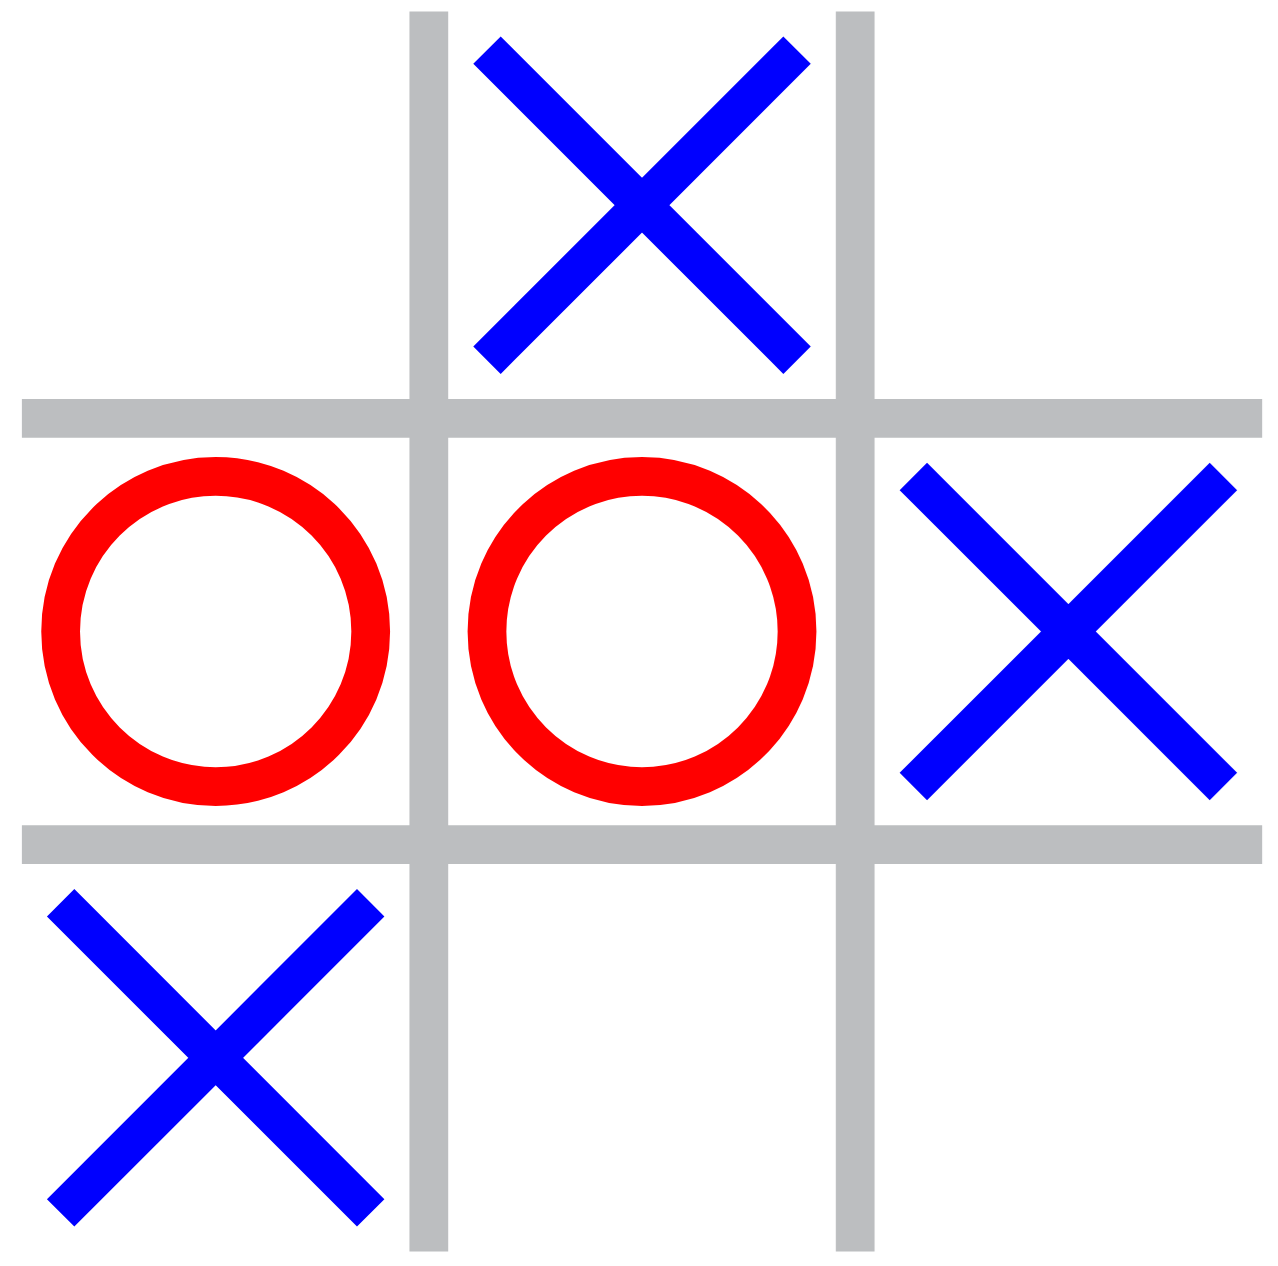
\includegraphics[width=0.4\linewidth]{figures/tictactoe.png}        

    
    \uncover<2>{Player 1 can almost-surly enforce a tie.\\}
    \uncover<2>{Player 2 cannot.\\}
\end{figure}
\end{frame}


\begin{frame}[label=conclusion]{Conclusion and Future Work}
\begin{columns}
\column{.5\textwidth}
Conclusion
\begin{itemize}
    \item Algorithm for qualitative reachability
    \item Proof of correctness
    \item Performant implementation in Storm
    \item Evaluation
\end{itemize}
\column{.5\textwidth}
\uncover<+->{Future Work}
\begin{itemize}
    \item Quantitative Checking / Value Iteration
    \item Symbolic Representation
    \item Optimization using MDP Algorithms
\end{itemize}
\end{columns}
\end{frame}